% SECTION: Probabilistische PCA
\section{Probabilistische PCA}

\divider

% SUBSECTION: PPCA Modell
\subsection{PPCA Modell}

% PCA als latent Variable Model
\begin{frame}{PCA als latent Variable Model}{}
	\begin{itemize}
		\item Wir modellieren die Repräsentation der Daten im Principal Subspace als latente Variablen $\bz \in \R^D$.
		\item Für die Verteilung von $\bz$ gelte
		\begin{equation} \label{eq:ppca-dist-z}
			\bz \sim \norm(\0, \bI).
		\end{equation}
		\item Zudem führen wir die bedingte Verteilung von $\bx \in \R^M$ gegeben $\bz$ wie folgt ein
		\begin{equation} \label{eq:ppca-dist-x-given-z}
			\bx \mid \bz \sim \norm\bigl( \bW \bz + \bmu, \sigma^2 \bI \bigr).
		\end{equation}
		\item Die Spalten der Matrix $\bW \in \R^{M \times D}$ spannen hierbei den Principal Subspace auf.
		\item Es ist $\bmu \in \R^M$.
		\item Der Parameter $\sigma^2$ beeinflusst die Varianz der bedingten Verteilung \eqref{eq:ppca-dist-x-given-z}.
	\end{itemize}
\end{frame}


% PPCA als generatives Modell
\begin{frame}{PPCA als generatives Modell}{}
	Die PPCA kann als \textit{generatives Modell} aufgefasst werden:
	\begin{itemize}
		\item Zunächst wählen wir ein $\bz$ gemäß \eqref{eq:ppca-dist-z}.
		\item Dann ziehen wir die beobachtete Variable $\bx$ aus der Verteilung \eqref{eq:ppca-dist-x-given-z}.
		\item Hierbei ergibt sich der Wert für $\bx$ gemäß
		\begin{equation} \label{eq:ppca-comp-x}
			\bx = \bW \bz + \bmu + \bepsilon.
		\end{equation}
		\item $\bepsilon$ ist hierbei \textit{additives normalverteiltes Datenrauschen},
			welches durch den Parameter $\sigma^2$ in \eqref{eq:ppca-dist-x-given-z} modelliert wird.
	\end{itemize}
	
	\begin{boxGray}
		\textbf{Bemerkung:} Die umgekehrte Sichtweise, also das Mapping der beobachteten Daten in den Principal Subspace,
		erhalten wir hieraus in Kürze mit dem Satz von Bayes.
	\end{boxGray}
\end{frame}


% PPCA als generatives Modell (Forts.)
\begin{frame}{PPCA als generatives Modell}{}
	\begin{figure}
		\centering
		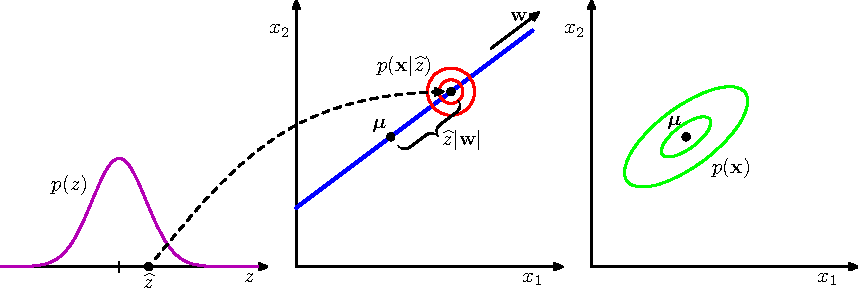
\includegraphics[scale=0.9]{./img/ppca/ppca_generative}
		\caption{PPCA als generatives Modell. Siehe \cite{Bishop2006}, Seite 572.}
	\end{figure}
\end{frame}